\part{Distributed Formation}

\chapter{Local Attachment Rules and What a Cluster Establishes}

\section{From a Rule to a Cluster}

Part V studies structures that form without a plan: no part of the structure is placed by a global design, and its shape results from many local events governed by a rule. The first such rule is the simplest one that already produces a surprising object. A single site is occupied. Particles arrive one at a time, wander at random, and stop when they touch the structure. After a few thousand arrivals the structure is a branching cluster with long arms and deep fjords, nothing like the compact blob that a naive picture of random deposition suggests. The process is called diffusion-limited aggregation, and it is used here because it is small enough to state completely and rich enough to show what a simulation can and cannot establish.

A rule is complete only when everything that affects the outcome has been stated. For the version used here the statement is as follows. The sites are the integer points of the plane, and the seed occupies the origin. Each walker starts on a circle of radius $r+5$ about the origin, where $r$ is the distance of the farthest occupied site, at the lattice point nearest a uniformly random angle. It moves one step along a coordinate axis, in one of the four directions with equal probability. If it ever stands at a distance greater than three times its launch radius from the origin it is discarded. If it stands next to an occupied site it joins the cluster with probability $p$, the stickiness, and otherwise continues. Seven things in that paragraph are choices: the lattice, the neighbourhood, the launch radius, the kill radius, the step distribution, the sticking probability, and the random number generator with its seed. Some of them are expected to matter for the result and some are expected not to, and the point of the chapter is to find out which, by measurement.

\section{The Rule as Code}

The rule is short enough to read in full.

\Needspace{26\baselineskip}
\lstinputlisting[language=Python,basicstyle=\ttfamily\footnotesize,breaklines=true,frame=single,columns=fullflexible,keepspaces=true,firstline=9,lastline=32]{dla.py}

This version uses Python's own generator and a set of occupied sites, and it is slow, because a walker from a distance $R$ needs of the order of $R^2$ steps to reach the cluster. The file \texttt{dla.py} also contains a version compiled with the Numba package that follows the identical rule on an array, and the ensembles below use it. The two versions use different random number generators, so they do not produce the same clusters from the same seed, and the check is statistical. With $10$ seeds each at $N=700$, the exponent defined below was $1.737\pm0.118$ for the Python rule and $1.692\pm0.101$ for the compiled one, where the figures after $\pm$ are standard deviations across seeds. The difference, $0.045$, is within one standard error of the difference, $0.049$, so the two versions agree to the precision of the test.

Reproducibility inside one version was checked directly: the same seed gave the same cluster, site for site, and a different seed gave a different one, with only $233$ of $1500$ sites shared between seeds $5$ and $6$, mostly in the early core. The first five sites of seed $5$ were $(0,0)$, $(0,1)$, $(0,2)$, $(0,3)$, $(1,3)$. A cluster is therefore a function of the rule, its parameters, the seed, and the version of the generator, and a record that omits any of these does not reproduce it.

\section{What the Cluster Is}

The standard summary of a cluster is its mass--radius relation. If the first $n$ particles have radius of gyration $R_g(n)$, the root-mean-square distance of the particles from their centroid, a compact cluster of the plane would have $n\propto R_g^2$ and a one-dimensional string would have $n\propto R_g$. A branching cluster has an exponent between, called its fractal dimension $D$:
\[
  n\;\propto\;R_g^{\,D}.
\]
The exponent was estimated by a least-squares line of $\log n$ against $\log R_g$ at $24$ logarithmically spaced values of $n$ from $100$ to $3000$. Over $20$ seeds, each with $3000$ particles, the estimate was $D=1.713$ with a standard deviation across seeds of $0.068$ and a standard error of the mean of $0.015$. Individual clusters gave values from $1.594$ to $1.838$. The radius of gyration at $3000$ particles was $51.8$ with a standard deviation of $1.4$. The value is close to the $1.71$ usually quoted for planar aggregation of this kind in the literature, a comparison recalled from reading and not tested here.

The variation across seeds is the first thing to notice. A single cluster gives $D$ within about $\pm0.07$ of the mean, so a statement of the form ``this cluster has dimension $1.84$'' would be wrong by an amount that is easily mistaken for a property of the model. The standard error of the mean over $20$ seeds, $0.015$, is a statement about the estimator, and it does not include the systematic effects below.

\section{The Fit Window}

The estimated exponent depends on the range of cluster sizes used for the fit. The same $20$ clusters were refitted over different windows.

\begin{center}
\begin{tabular}{rrr}
\toprule
Fit window in $n$ & Mean $D$ & sd across seeds\\
\midrule
20 to 200 & 1.680 & 0.118\\
100 to 600 & 1.691 & 0.105\\
200 to 1000 & 1.726 & 0.108\\
500 to 3000 & 1.728 & 0.069\\
1000 to 3000 & 1.733 & 0.064\\
100 to 3000 & 1.713 & 0.068\\
\bottomrule
\end{tabular}
\end{center}

The estimate drifts upward by about $0.05$ as the window moves to larger clusters, which is more than three standard errors of the full-window value. The drift is a systematic effect: small clusters have not yet developed their branching, and a line fitted through them has a different slope. A report of $D$ should state the window, and the honest summary of this experiment is that $D$ is between $1.68$ and $1.73$ depending on the window, at these sizes. Whether it continues to drift at larger $n$ was not tested.

\section{The Lattice Leaves a Signature}

The rule is stated on a square lattice and the continuum process it stands for has no preferred directions. A measurement can ask whether the lattice shows. For the outer half of each cluster, that is the particles beyond half the largest radius, the amplitude of the $m$-fold angular harmonic $|\langle e^{im\theta}\rangle|$ measures how much the particles favour $m$ directions. For $m=4$ the amplitude, over $20$ clusters of $3000$ particles with about $1440$ outer particles each, was $0.295\pm0.115$ (standard deviation across seeds), against $0.024\pm0.012$ for an isotropic cloud of the same size. The four axis directions are strongly preferred, by a factor of about twelve in amplitude. The two-fold amplitude was $0.235\pm0.138$ and the eight-fold $0.171\pm0.064$, so single clusters are lopsided as well. The axis-aligned arms visible in the left cluster of Figure 15.1 are consistent with this.

This is the limit that most affects what the cluster may be used for. A conclusion about the geometry of branching in general would need the same rule off the lattice, with continuous positions, and the dimension quoted above is a property of the lattice rule. A conclusion about how a branching rule turns local contact into global shape is supported by the experiment, because the lattice is a way of making the rule precise and not a feature that the conclusion depends on.

\section{Stickiness}

The sticking probability $p$ was varied over four values with $12$ seeds each at $N=2000$ and the same fitting procedure, using the window $100$ to $2000$.

\begin{center}
\begin{tabular}{rrrr}
\toprule
$p$ & $D$ (mean $\pm$ sd) & $R_g$ at $N=2000$ & Run time (s)\\
\midrule
1.00 & $1.765\pm0.101$ & 41.2 & 3.9\\
0.50 & $1.727\pm0.088$ & 34.7 & 2.7\\
0.10 & $1.730\pm0.115$ & 22.7 & 1.9\\
0.02 & $2.078\pm0.133$ & 13.6 & 1.4\\
\bottomrule
\end{tabular}
\end{center}

The radius of gyration at fixed $N$ falls steadily with decreasing stickiness, from $41.2$ to $13.6$, so the clusters are visibly more compact. Over the range $p=1$ to $0.1$ the exponent is the same within the scatter, standard errors being near $0.03$, so stickiness changes the size of the cluster for a given number of particles and no change in $D$ was detected. At $p=0.02$ the fitted value, $2.08$, exceeds the dimension of the plane, which no cluster in the plane can have, and so the number is not a dimension at all. The likely reason is that at low stickiness particles penetrate and fill the interior before branching starts, so in this window the cluster is compact at small $n$ and branches at larger $n$, and one straight line through the whole range is the wrong model. That interpretation is an explanation of the number and was not tested by extending the range. The lesson is that a fitted exponent is meaningful only where the data lie on a line, and an exponent outside the physically possible range is a diagnostic that the fit is wrong.

Figure 15.1 shows two clusters from the same seed, $2000$ particles each, with $p=1$ on the left and $p=0.1$ on the right, coloured by arrival order. The radii of gyration are $38.6$ and $21.9$.

\begin{figure}[ht]
\centering
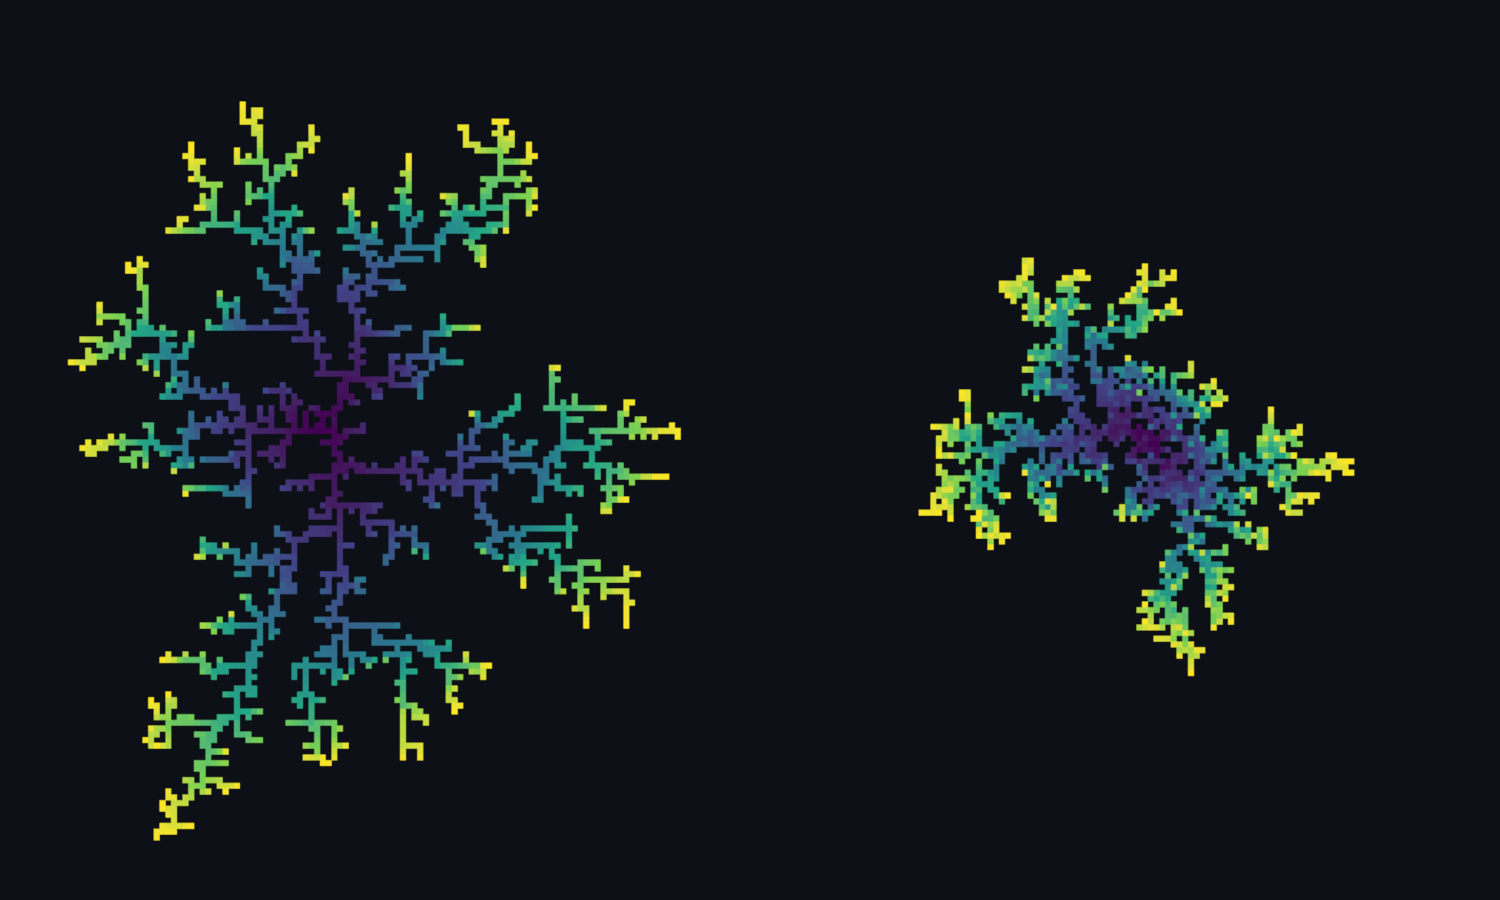
\includegraphics[width=\textwidth]{figs/fig15_clusters.png}
\caption{Two clusters of $2000$ particles with the same seed, $p=1$ (left) and $p=0.1$ (right), viewed from above in Blender with one material that colours each cube by its arrival order, from early (purple) to late (yellow). The radii of gyration are $38.6$ and $21.9$.}
\end{figure}

\section{The Cluster in Blender}

The cluster is brought into Blender as a collection of objects that share one cube mesh, one object per site, in the manner of Chapter 5, with the arrival order stored on each object as a custom property. One material, built as in Chapter 8, reads the property with an Attribute node and maps it through a viridis colour ramp, so the whole cluster uses a single material. The script is \texttt{dla\_blender.py}. For a cluster of $1000$ particles from seed $7$ the scene held $1000$ objects at $1000$ distinct sites, one mesh with $1000$ users, and one material. Every site after the first was adjacent to an earlier one, so the scene is a connected cluster that grew in the recorded order and not a cloud of points; all positions were integers; the stored order matched the creation order; and the seed and stickiness recorded on the collection regenerated the same cluster, site for site. The scene is thus checkable against its own provenance, which is the standard the preceding chapters set for a generated structure.

\section{What the Experiments Do Not Show}

All results are for clusters of at most $3000$ particles on a square lattice, with at most $20$ seeds per condition. The launch offset of $5$ and the kill radius of three launch radii are modelling choices whose effect was not tested, and either could bias the clusters, for instance by discarding walkers that would have reached the tips. The step distribution, the four-neighbour rule, and the generator were not varied. The exponent estimates describe these finite clusters over the windows stated and do not support a claim about the infinite limit. The comparison with the literature value is from recollection. Nothing here shows that a physical process of any particular kind, such as mineral growth, electrodeposition, or the branching of a colony, follows this rule. The experiment shows what the rule does, with a stated precision, and a claim about a physical system would need a separate test of the rule against it.

\begin{exercise}[15.1: Vary the kill radius]
Repeat the dimension estimate at $N=2000$ with kill radii of $2$, $3$, and $5$ launch radii, using $12$ seeds each, and report whether the exponent or the radius of gyration changes by more than the standard error.
\end{exercise}

\begin{exercise}[15.2: Find the crossover]
At $p=0.02$, compute the local slope of $\log n$ against $\log R_g$ in windows of a factor of two in $n$, up to $N=6000$, and describe where the slope crosses from $2$ toward a smaller value.
\end{exercise}

\begin{exercise}[15.3: Off the lattice]
Implement the rule with continuous positions, particles of unit diameter, and sticking on contact, and repeat the harmonic analysis of Section 15.5. State how the four-fold amplitude changes and what that says about the lattice's role.
\end{exercise}

\begin{exercise}[15.4: A record that reproduces]
Write the minimum record from which a cluster in a scene can be regenerated, test it by regenerating from the record alone, and then change one element of the record, such as the version of the generator, and describe what fails.
\end{exercise}
